\documentclass[UKenglish]{uiomasterthesis}
\usepackage{graphicx} % Required for inserting images
\usepackage[UKenglish]{uiomasterfp}
\usepackage[nottoc]{tocbibind}
\usepackage[hidelinks]{hyperref}
\title{Explainable Reinforcement Learning}
\subtitle{Discovering intent based explanations for heterogeneous cooperative multi agent reinforcement learning agents}
\author{Ada Hatland}
\date{August 2024}
\begin{document}
\uiomasterfp[master, program={Informatics: Robotics and Intelligent Systems},
  color=orange, dept={Department of Informatics}, fac={The Faculty of Mathematics and Natural Sciences},
  supervisors={Dr. Dennis Gro\ss \and Prof. Kyrre Glette\and Dr. Helge Spieker}, image =  {images/b1efc86c-d976-43a3-92e3-753ef0e114b0}]


\tableofcontents

\chapter{Introduction}

Sequential decision-making problems, where one decision leads to a new state that requires a new decision to be made. An example of this is autonomously driving from point A to point B through city streets. For these types of problems Reinforcement Learning (RL) systems are used. RL, both multi- and single-agent models have seen a significant rise in successful use and applicability in recent years, with models like AlphaGo\cite{article} and smacv2\cite{ellis2023smacv2}. These models learn by agents performing actions in a given state decided by a policy that lead to a new state, and learning by receiving rewards depending on if the new state is preferable to the previous, the aim is to learn a near optimal policy for achieving a fixed goal\cite{Sutton1998}. The agent uses an observation of the state to choose an action. The environment describes how an action affects the state. See Figure 1. In a Multi-Agent Reinforcement Learning (MARL) system, we would have multiple agents.

\begin{figure}[!ht]
	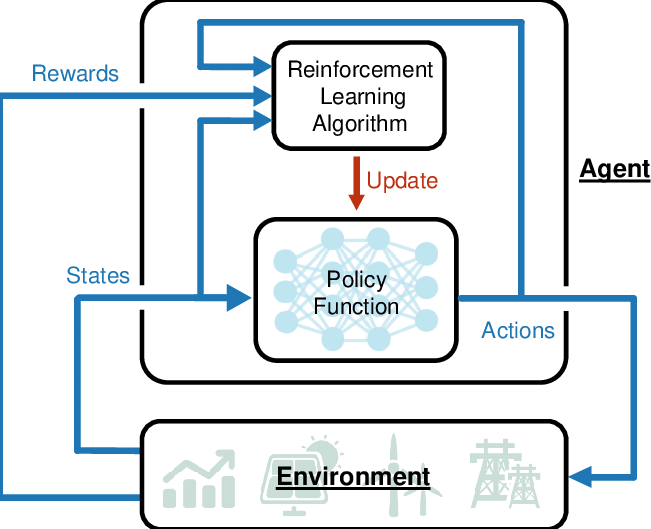
\includegraphics[width=\columnwidth]{images/Basic-structure-of-reinforcement-learning-The-agent-can-observe-the-states-of-the.png}
	\caption{Structure of a simple RL system as found in Review of Learning-Assisted Power System Optimization \cite{unknown}}
	\label{fig:environment}
\end{figure}

A significant problem with many deep machine learning models, including MARL policies, is known as the black box problem\cite{zednik2019solving}. This problem describes how the processing of information is hidden from a human user due to the opacity of the model, and we just have to trust that the model uses relevant data to come to the conclusion it does, which it often doesn't do. For many tasks and models where the impact of the output isn't highly significant this isn't a big issue, but for tasks like autonomous driving we simply cannot use these models without trust for the models processing of data and that the solution given wont hurt anyone. We can considering autonomous driving as a MARL system if we consider each vehicle as an agent. To solve this we would like to have models that along with an output can provide us with some kind of reasoning for what information is used and how.

All this essentially means, until the black box problem is solved, autopilot will always require a driver behind the wheel\cite{tian2018deeptest}. Despite having high accuracy, precision and recall, a reinforcement learning model might choose a less than preferable action in edge cases or states not well covered by training and test sets, for example driving on snowy roads when all images in the training data is from warmer climates, or combinations that aren't well covered, like a foggy, snowy road with a sharp right turn.
With a way to ask the agent for intent, we could find that it has learned to always expect there to not be a car around the corner, which is not always obvious from looking at the dataset, but if it in a decision relies on the road to be empty to choose a safe route, this is obviously a huge issue. This paper aims to explain how an agent in a MARL setting decides on an action due to what it expects from other agents in the future. The field working on combating this issue is known is Explainable reinforcement learning.

Explainable Artificial Intelligence (XAI) is an umbrella term for all explainable artificial intelligence. The focus of this paper will be to rework and apply methods for general XAI to Reinforcement Learning (XRL). In particular we will focus on an agent and how the expected future states of other agents will affect it in its decision making process. The environment we will focus on is a MARL environment known as Knights Archers Zombies \cite{KAZ} made for Python. We use this because it is a cooperative environment where each agent has to consider other agents, both of the same type as itself, and other types. If we used an environment where all the agents are identical, our findings will be less useful for other environments where the agents aren't identical. In many real life scenarios agents will not be identical. If we once again consider autonomous vehicles, most vehicles are different in some way. A very obvious example of this is considering cars and motorcycles. Where because of their size difference, their paths chosen will often be different.

In psychology it is well known that most human based decisions are made with intent\cite{inbook}, and by focusing on the expectation of what future states will look like we can consider this the intent of the agent. If we are accurately able to extract the intent of an RL policy we are better able to explain the choice made and we are more comfortable with trusting that the choice made is a good decision.

We aim to construct a framework to describe the intent of the agents in the KAZ environment, and we aim to make it applicable to other environments as well. First we will go a bit more in depth on what type of explainablity we want to use as well as describe relevant methods already used, then we will attempt to integrate previous and own methods into a MARL policy we construct and train, and at the end we will discuss our findings.

\medskip
\chapter{Background}

\section{Post hoc vs. intrinsically explainable models}
This section will discuss benefits and drawbacks of explainable models divided into two main categories, Post hoc models and intrinsically explainable models.

Post hoc explainability refers to finding ways to understand already trained models. Instances where this doesn't pose more of a challenge can often be more efficient as you do not need to construct and train a model, which could often pose an issue both considering time spent and accuracy of the model. Making a model explainable only makes sense if we know it usually makes sensible decisions. There are however issues with making post hoc models.

\subsection{ Temporal aspect}
RL policies all have a temporal aspect, which means several different actions over a certain period of time might contribute to a singular outcome, this could make it very challenging to pinpoint which actions were made for which outcome, especially if the outcome happens several states after the initial decision was made.

\subsection{ Nature of black box models}
Many RL policies, especially deep RL policies, which are the policies we will be working with, have complex inner connections due to the hierarchical structure of learning features in the input, sequences of non linear connections that are very hard to understand without spending a lot of time studying the specific connections learned by a model. It's often very difficult to accurately pinpoint the purpose of a node, especially because we do not know if it even has a purpose at all or it could have a lot of different purposes. Especially in environments with complex observation spaces.


\subsection{ Lack of transparency}
Tracing how an observation leads to a state, through the action chosen and the environment, is often challenging in models constructed without this in mind. If we do not know the processing of information of a model it's very hard to explain the rationalisation of an agent.

\subsection{ Intrinsically explainable models}
Intrinsically explainable models has the aforementioned drawback of relying on model construction to be done well, as we will be unable to use a model that is shown to be accurate, but since it doesn't get as affected by point II.I to II.III it will be the preferred method in this paper.


\medskip

\section{Fidelity of XAI methods}
It is important to understand why the current XAI methods not meant for RL applications aren't always useful to us.

XAI methods not intended for reinforcement learning often provide\\ explanations that don't necessarily represent the inner workings of an RL policy, because an RL policy has a temporal aspect as well. Broadly these methods can be categorised as feature-based explainers, and they often struggle to fully explain an agents behaviour or specific actions because they cannot capture the future view of an RL policy. 

Saliency maps which have been successfully used for classification of images provide explanations about what part of the input was important for the outcome, which is highly relevant for classification tasks, but using the same method for an RL policy doesn't sufficiently explain the intent of the agent\cite{atrey2020exploratory}.

Another commonly used XAI method is model distillation, which works by transferring knowledge from a large model to a smaller, usually interpretable, one, for instance a deep learning network to a decision tree \cite{bastani2019verifiable}. This has use cases in verifyability, but struggles to fully explain the temporal aspect of RL policies, and are therefore not sufficient as an explainer.

However, these methods might still prove insightful in conjunction with other intent-based methods, the state in which a decision is made is obviously very relevant to why that particular decision was made. We could perhaps use these methods to answer questions such as "What part of agent As Observation this state, lead it to believe agent B would end up at these coordinates at a later state?"
\medskip

\section{Future-based explanations}
Next, I will describe in slightly more detail, what is meant by an intent based explainer, like I want to develop, and how to use it.

\subsection{ Design}
"Towards Future-Based Explanations for Deep RL Network Controllers"\cite{10.1145/3626570.3626607} broadly describes future-based intrinsically explainable methods. Future-based intrinsically explainable methods for DRL policies often take three inputs, the trajectories experienced by an agent, the environment and the agent. Then, they collect the rewards and interactions and use this information to train an explainer.

During inference, we can then apply the explainer to a state and action to get the expected future consequences of that action. Depending on the architecture we could either get the expected future consequence of any action, or just the one the agent decides on.

\subsection{ Use cases}

Designing a DRL solution requires choosing features in the observation,\\ hyperparameter tuning, policy design and reward function among other things. This is a time, and resource, consuming process. These are usually picked by trial-and-error but could be made easier with assistance from an explainer. See Figure 2. 

Another, and perhaps more important, use case is safety. If when online, i.e. the chosen action will actually affect the state, we are expecting high likelihood of an unsafe state, we could instead of opting for the chosen action fall back to a known safe action, that could have a lower expected return, i.e. breaking instead of turning a corner if we have limited vision around the corner.

\begin{figure}
	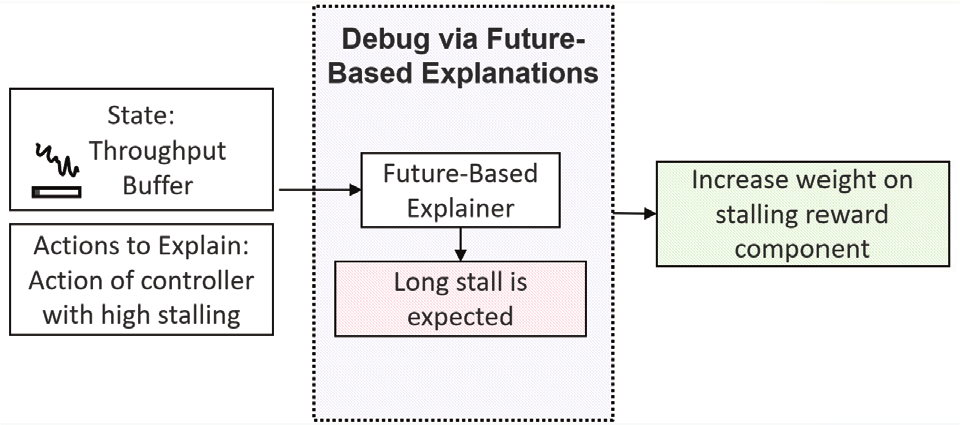
\includegraphics[width=\textwidth]{images/dog-final.png}
	\caption{Using a future-based explainer as debugger to avoid stalling for adaptive bitrate streaming as found in "Towards Future-Based Explanations for Deep RL Network Controllers" \cite{10.1145/3626570.3626607}}
	\label{fig:environment}
\end{figure}
\medskip

\subsection{Definition of intent}
We define the state transition function $T(s, \textbf{a}, s')$ where $\textbf{a}$ is the set of simultaneous actions made by the set of active agents, in our case, one action per agent. Given $T$ the agent should when prompted output a set of trajectories $\tau = \{(s_0,\textbf{a}_0),(s,\textbf{a}),(s_1,\textbf{a}_1)...(s_n,\textbf{a}_n)\}$ where $s_0$ is the current state, $\textbf{a}_i$ is the set of actions taken in $s_i$, and $s_{i+1}$ is the state reached by $T(s_i,\textbf{a}_i, s_{i+1})$. We define these sets of trajectories, along with their probabilities believed by a certain agent $A$, as the intent of the agent. The agent $A_0$ only has information about $a_0$ in the set $\textbf{a}$.

How do we separate intent of 1 one and agent 2

Extract intent from trajectory, start with reward


\section{Relevant methods}
There are several papers written on XAI and XRL problems. Milani et al.\cite{milani2022survey} categorise XRL into three main categories, feature importance (FI), learning process and MDP (LPM) and Policy-level (PL). FI considers the immediate context for actions, i.e. what part of the input was important for a single action, LPM considers techniques that highlight which experiences in training were influential for the final policy and PL focuses on long term effects and behaviour. Since we are interested in future states and actions we will look at influential trajectories and transitions within these trajectories. It is important to view these transitions in the context of the trajectory to understand the long term effects and not just immediate, which are of less interest in this paper, if we find the state with a high state importance $I(s)$, $I(s) = max_aQ(s,a)-min_aQ(s,a)$ most similar by some similarity measure to an arbitrary current state we could find the resulting trajectory and expect the agent to intend a similar outcome. There are also ways to convert Recurrent Neural Network (RNN) policies to an interpretable models post-hoc, which might be relevant if we use an RNN. This paper will explore PL explainability further.

In particular "What did you think would happen? Explaining Agent Behaviour through Intended Outcomes" \cite{yau2020did}, "Explainable Reinforcement Learning via a Causal world model" \cite{yu2024explainable} and "CrystalBox: Future-based explanations for input-driven deep RL systems" \cite{patel2024crystalbox} are highly relevant due to the fact that they all describe temporal connections between current actions and future states or actions.

"Are large language models post-hoc explainers" \cite{kroeger2024large} Could be relevant as using other explainers to compare explanations is useful. "ACTER: Diverse and Actionable Counterfactual Sequences for Explaining and Diagnosing RL Policies" \cite{gajcin2024acter} 

\subsection{ What did you think would happen? Explaining Agent Behaviour through Intended Outcomes}
What did you think would happen describes what an agent expects to happen in future states, and why the current action is chosen based on the future expectations. As stated in the paper, a limitation of their method means it doesn't work well with high dimensionality. The two main difference between this paper and the problem i aim to solve is that they're focusing on an environment with a single agent and that our observation space will be high dimensionality. It uses Q-learning and Markov-chains that train simultaneously with a "belief map" that shows what the agent expects the environment to look like in future states. In the simple examples used in the paper it shows where it believes the taxi should drive and therefore chooses an action to follow this path. This is not directly applicable to my thesis as it's unlikely that Q-learning or Markov chains will be viable for the intended model based on the environment. However the paper is successful in explaining an agents underlying motivations and beliefs about the causal nature of the environment, and using similar methods might be an effective means for making MARL agents with higher dimensionality understandable from a human perspective.

\begin{figure}[!ht]
	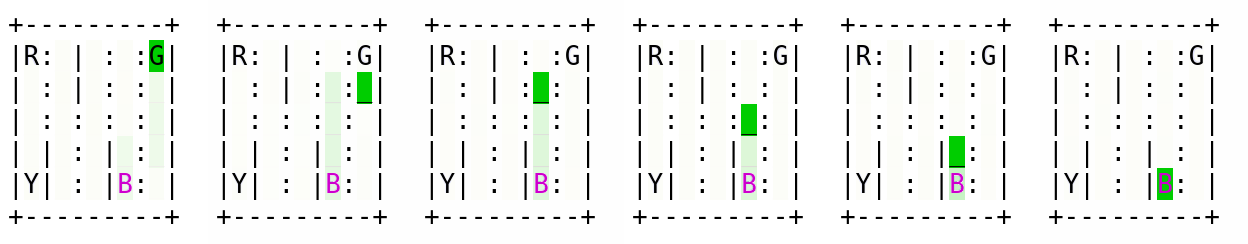
\includegraphics[width=\columnwidth]{images/merged_14_dqntaxi.png}
	\caption{Belief map of a Taxi driving from G to B, where the opacity describes the likelihood of the taxi entering that square as found in "What did you think would happen? Explaining Agent Behaviour through Intended Outcomes" \cite{yau2020did}}
	\label{fig:environment}
\end{figure}

\subsection{ Explainable Reinforcement Learning via a Causal world model}
Explainable Reinforcement Learning via a Causal world model constructs a sparse model to connect causal relationships, without prior knowledge of the causal relationship, rather than a fully connected one, but they still achieve high accuracy and results comparable to other fully connected Model-Based Reinforcement Learning (MBRL) policies. Which is important, as there is often a trade off between explainability and performance. Using the same model for both explanations and choosing actions also make the explanations faithful to the intentions of the agent. The paper also describes a novel approach to derive causal chains from the causal influence of the actions, which lets us find the intent of the agent. The paper is successful being applied to MBRL, and is also applicable to models with infinite actions spaces, which is a limitation of some other models, see previous sub section.

A limitation of the paper is that it requires a known factorisation of the environment, denoted by $\langle S, A, O, R, P, T, \gamma \rangle$, where S is state space, A is action space, O is observation space, R is reward function, P is probability function for the probability of transitioning from state $s$ to state $s'$ given action $a$, T is the termination condition given the transition tuple $(s,a,o,s')$, and $\gamma$ is the discount factor. Considering we will be working with hand crafted simulations we will have access to all of these, however its not certain that if we depend on this method that our contributions will be applicable to certain other environments where the factorisation is not known.


\subsection{ CrystalBox: Future-Based Explanations for \\Input-Driven Deep RL Systems}
CrystalBox introduces a model-agnostic, post-hoc, future based explanation for DRL. It doesn't require altering the controller, and works by decomposing the future rewards into its individual components. While this isn't exactly the kind of explanation we are looking for, it could be a great tool in developing an explainer that considers other agents actions in a multi agent cooperative environment, which is the goal of our paper, because it is post-hoc, and easily deployable. Especially because it was constructed for input-driven environments. The original paper claims it offers high fidelity solutions for both discrete and continuous action spaces. KAZ has a discrete action space but we might do some work with other environments as well.

It's not certain to be useful because it works by decomposing the reward function, and it's not safe to assume the reward function will even be useful to decompose.


\subsection{ Are Large Language Models Post Hoc Explainers}
A Large Language Model (LLM) is a predictive model that generates text based on a prompt you give it, be it continuing the prompt or responding, and can often give the impression of comprehension of human language and a deeper understanding of the topic at hand.  The paper aims to investigate the question "Can LLMs explain the behaviour of other complex predictive models?" by exploiting the in-context learning (ICL) capabilities of LLMs. ICL allows LLMs to perform well on new tasks by using a few task samples in the prompt. A benefit of using an LLM as a post-hoc explainer, is that the output given by the model will already be written in natural language and should be understandable by a layman. The paper presumes that the local behaviour of a model is a linear decision boundary, and by using a sample x and perturbing it to x', and presenting both the samples and the perturbation as natural language we could get an explanation from the LLM for the outcome. With a sufficient number of perturbations in a neighbourhood around x the LLM is expected to explain the behaviour in this neighbourhood, and rank the features in order of importance.

While the faithfulness of the LLM as an explainer is on par with other XAI methods used for classification, meaning that the reasons provided are enough to explain the output, I am sceptical of the fidelity of the LLM for two reasons. One is the same as for why other XAI models often struggle with fidelity, the temporal aspect. If applied in the same way as in the paper it would not consider the intent or the past and only what part of the current observation made it make a certain decision. The other is that I am sceptical of claims presented by an LLM in general as these are all just guesses. Good guesses a lot of the time, but still just guesses. 

We could however potentially change the implementation so it considers the temporal aspect, and this might be a viable post hoc explainer after some more research into prompt engineering.


\subsection{ ACTER: Diverse and Actionable Counterfactual\\ Sequences for Explaining and Diagnosing RL Policies}
The paper presents ACTER, an algorithm that uses counterfactual sequences with actionable advice on how to avoid failure for an RL policy. It does this by using an evolutionary algorithm (EA) known as NSGA-II to generate counterfactual sequences that don't lead to failure as close as possible to factual sequences that lead to failure. This paper presents counterfactual sequences and not just actions, which means it also presents how to avoid the state that lead to failure to begin with, which should, if ACTER is implemented correctly, allow us to significantly reduce the amount of times our policy fails. It also offers multiple counterfactuals to allow the end user to decide which counterfactual is preferable to their use case.

There are 4 hypothesises tested by the paper. The last two considers laymen users and are therefore not as interesting to us. The first two however "ACTER can produce counterfactual sequences that prevent failure with lower effort and higher certainty in stochastic environments compared to the baselines." and "ACTER can produce a set of counterfactual sequences that offer more diverse ways of preventing failure compared to the baselines." are partially and fully confirmed respectively. Which means ACTER will likely be a useful tool to explain and diagnose our RL policy.


\medskip
\chapter{Methodology}
\section{--IPPO vs MAPPO}
Using IPPO for now because \cite{dewitt2020independentlearningneedstarcraft}. Should be enough for explainability.

\section{--Formally define intent}
Intent vs. goal?

We define the intent of an agent as the short term goal.

Some knowledge of the state transition function

Expectation of other agents actions.


\section{--Reward function changes?}

\section{--How to identify intent}

\section{--Synergy/intent collision}
Cooperation index

\section{--Lazy agents/sparse rewards}
archers train fine, knights only start learning anything useful after a very long time, ~12M timesteps, then not stable

-alternate reward structure?

-memories to focus more on knights?

-policy architecture?

-start with only training knights at first then add archers as well? (eg. 4 knights -> 2 knights, 2 archers) for consistent action and observation space. Similar to using a reward structure where only knights gain rewards for n timesteps before both knights and archers gain rewards. 

-Possible to not have the same reward for every agent, but then no centralised critic

\section{--Same intent for same state? Different policies?}
Swap homogeneous agents to see intent difference

\section{--Change environment, related to permutation importance}

\section{--Feature importance}
Detect which zombies agents care about
saliency maps

\section{--Feature permutation changes, for other agents and zombies}
\bibliography{ref}{}
\bibliographystyle{unsrt}
\end{document}
